% Created 2022-10-07 Fri 18:05
% Intended LaTeX compiler: pdflatex
\documentclass[a4paper,12pt]{article}
\usepackage[utf8]{inputenc}
\usepackage[T1]{fontenc}
\usepackage{graphicx}
\usepackage{longtable}
\usepackage{wrapfig}
\usepackage{rotating}
\usepackage[normalem]{ulem}
\usepackage{amsmath}
\usepackage{amssymb}
\usepackage{capt-of}
\usepackage{hyperref}
\usepackage[margin=1.0in]{geometry}
\usepackage{setspace} \usepackage[hyphens]{url} \usepackage{hyperref}
\date{\today}
\title{Predicting Lung Cancer with Machine Learning}
\hypersetup{
 pdfauthor={Alfred Nguyen},
 pdftitle={Predicting Lung Cancer with Machine Learning},
 pdfkeywords={},
 pdfsubject={},
 pdfcreator={Emacs 28.2 (Org mode 9.5)}, 
 pdflang={English}}
\begin{document}

\maketitle
\section{Introduction}
\label{sec:org95b9c50}
Lung cancer is the most common form of cancer in the world. Over 200.000 new cases are being diagnosed every year making up to 13\% of of all cancer diagnosis. Almost half of the patients with lungcancer die after a year after the diagnosis.
As for all forms of cancer, an early diagnosis increases the survival rate drasticaly. Earlier stages of lung cancer are easier to treat and can decrease the death rate by 14\% to up to 20\%[1].
Thus, applying machine learning, appears to be reasonable use case for the diagnosis of lung cancer, since it can achieve high effectivnes.

In this paper, I will try to determine whether a patient with certain characteristics has lung cancer or not.

\subsection{Report structure}
\label{sec:org74050f3}
The report will continue with the section 2, \emph{``Problem Statement''}, where the data set is presented and all the data points are clarified.
Section 3, \emph{``Methods''}, will explain how and why the feature selection was done and how the data sets were constructed.
Furthermore, the two machine learning methods, \emph{Logistic Regression} and \emph{Support Vector Machine (SVC)}, will be discussed.
In section 4, \emph{``Results''}, the results are evaluated and section 5, \emph{``Conclusion''}, will draw a final conclusion.

\section{Problem Formulation}
\label{sec:org0eaafe5}

\subsection{Data set}
\label{sec:orgc626aa8}
The data set consists of 309 entries in an Excel spreadsheet, with patients between 21 and 87 years old.
Each data point describes a patient with different characteristics.
The data set is licensed under the \emph{CCO: Public Domain} and was found on \emph{\href{https://www.kaggle.com/datasets/mysarahmadbhat/lung-cancer}{Kaggle}} [2].
For transparency, this dataset is used in another project found \emph{\href{https://www.kaggle.com/code/gaganmaahi224/lung-cancer-5ml-models-full-analysis-plotly}{here}} [3], but as this work was done independently, it has not been copied in any way.

The data set is complete and has no missing features. Each data point is mapped with 16 different attributes (gender, age, smoking, yellow fingers, chronic disease, \emph{see appendics for more}\ldots{}).
Additionally, I was also able to find 33 duplicates, which I have eliminated.
As you may have already noticed, the dataset is not too large, now containing only 276 entries. How this problem was dealt with will be further explained in the ``Data Splitting'' section.

\subsection{Label and feature clarification}
\label{sec:orgdde9a23}
The label for this prediction is whether a patient has lung cancer or not (yes/no), which means that this problem is a classification problem.
I decided to change the dataset for the labels from \emph{yes} and \emph{no} to \emph{-1} and \emph{1} to make the prediction easier and because I will use the SVC hinge loss function in the second part.
All attributes except gender and age are represented with \emph{1} or \emph{2}, which corresponds to \emph{no} and \emph{yes} respectively. The gender is represented with \emph{M} or \emph{F}, which means male or female respectively. The age is the actual age as an integer.
The histogram shows that the data is largely balanced, except for a few outliers such as \emph{fatigue} and \emph{lung cancer}. Since I will be using Logistic Regression, these outliers will not significantly affect our results [4][5].

\section{Methods}
\label{sec:orgd943626}
\subsection{Feature selection and engineering}
\label{sec:org3d0b17b}
For the features, I selected all attributes except for the lung cancer column, as it is used for the label. For the selected features, I have changed the data points from \emph{1} and \emph{2} to \emph{0} and \emph{1} for convention purposes and ease of understanding.
It is important to note here that with the exception of age, all characteristics can be represented in binary, meaning, a normalisation is not required.
After looking at the correlation heat map of the characteristic, I could not identify any bad data sets. All data points appear to be in the range of -0.75 and 0.75, which is a common indicator of correlation.
Also, all the identifiers, gender, age, smoking, yellow fingers, (\ldots{}) seem intuitively important in determining whether a patient has lung cancer or not.
After some manual tests with \emph{Variance Inflation Factor (VIF)} I could confirm that all 15 characteristics seem to improve the accuracy of the prediction.

\subsection{Data Splitting}
\label{sec:orgf92fcc7}
At first the data is split into two parts, the validation/training set and the test set. I chose the ratio to be 80 to 20 which was discussed in the lecture.
This helps us to split the whole data into two part, so that the test set is not used in neither the training set nor the validation set.
This was achieved by using the \emph{train\textsubscript{test}\textsubscript{split}} function of the \emph{sklearn} library.
The remaining part (80\%) of the data set will be used to train and validate the machine learning models.

As mentioned earlier, the data set is not very large.
I decided to use the k-fold cross-validation method. This method is suitable for data sets with fewer entries, to split it up into training and validation sets.
The algorithm works by randomly dividing the datasets into equal parts and using one set as the test set and the rest as the training set.
I decided to split the data into 5 parts (k=5) to achieve an 80 to 20 (training to validation) ratio, which is very common.
Our goal is to classify whether a patient has lung cancer. This can be described as a binary classification problem.

\subsection{Logistic Regression}
\label{sec:org4df2fe1}
For the first machine learning model, I chose Logistic Regression because it seemed reasonable for a simple binary classification problem.
Logistic Regression uses a linear hypothesis space and works by setting a limiter between the data points.
In a 2D space, you would put a line between the given data points. In 3D space, the points would be separated by a plane, and in higher dimensions you would use a hyperplane to describe the separation.

\subsubsection{Loss function for Logistic Regression}
\label{sec:orgd7be6f8}
For the loss function, I chose the Logistic Loss function, as it is a very common and proven function for Logistic Regression and was easy to use as it is already implemented in the used library.

\subsection{SVC}
\label{sec:org70cc6db}
For the second machine learning model, we chose to use the Support Vector Machine (SVM) classifier class, Support Vector Classification (SVC), for this simple binary classification task. For SVC, it also uses a linear hypothesis space that maps h(x) = w\textsuperscript{T}(x) , identical to that of the Logistic Regression method used previously. The decision to opt for this method was so that we can compare the classification methods and evaluate which has better performance. We did not choose to make use of LinearSVC or SGDClassifier over the basic SVC due to the dataset being not too large.
\subsubsection{Loss function for SVC}
\label{sec:orgd815911}

We also decided on using hinge loss to calculate the loss of our SVC method. The motivation for making use of hinge loss as the function for this method \% hinge loss function  ,\% is mainly because it is widely known as the loss function tailored for SVM and also is easily accessible with sklearn.metrics. Furthermore, it also makes sense to use this loss function for this binary classification task. A visualization and representation of the hinge loss function is shown in the following figures.


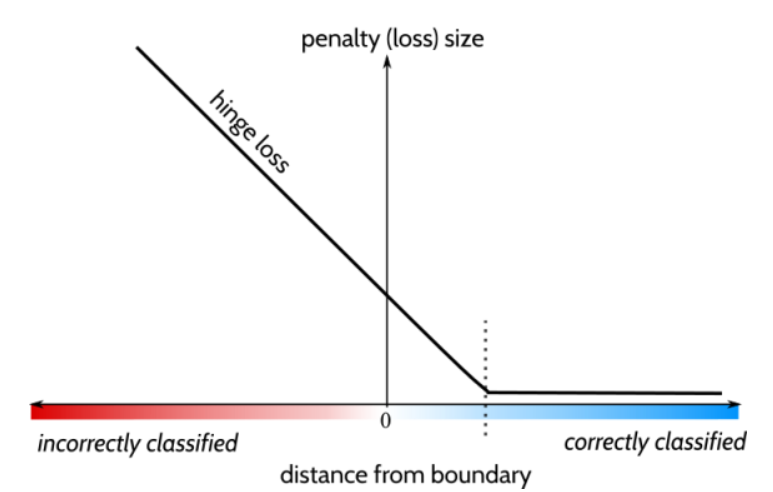
\includegraphics[height=0.3\textwidth]{./graphs/svc_1.png}
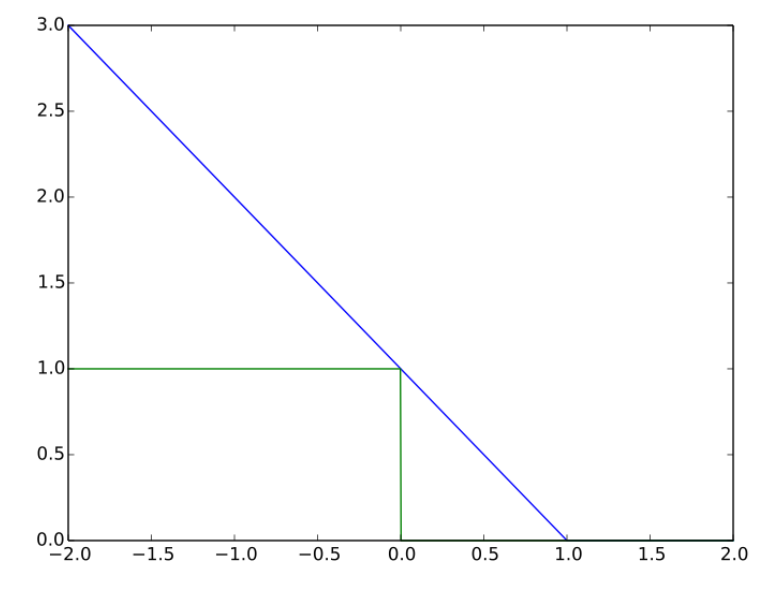
\includegraphics[height=0.3\textwidth]{./graphs/svc_2.png}


From these figures, we can see that for observations that are of a margin distance of greater than or equal to 1, the hinge loss is valued at zero. While for observations of margin distance less than 1, the hinge loss value incurs a loss the increases linearly. To put simply, while the SVC bears the similarity with Logistic Regression in that it aims to separate both classes with a line, the difference lies in this hinge loss function, that aims to maximize the margin distance between each data point and the separating line.

\section{Results}
\label{sec:orgcb52c55}

To evaluate and compare the two models, we have calculated the errors and the accuracy scores for each training, validation and test sets, obtaining the following results shown in the charts below.

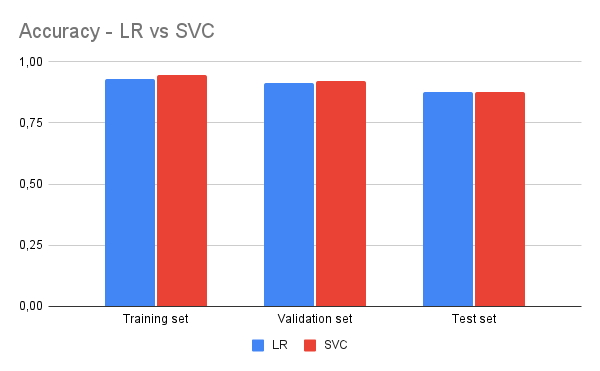
\includegraphics[height=0.3\textwidth]{./graphs/accuracy_chart.png}
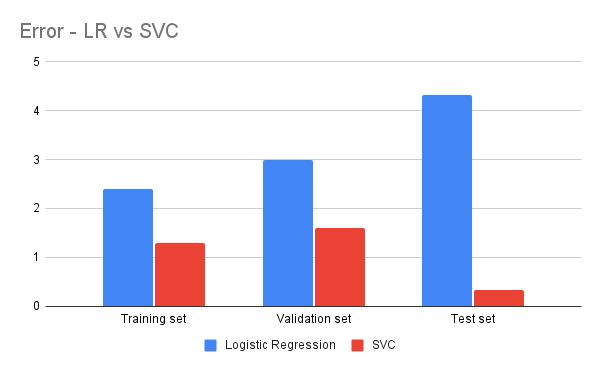
\includegraphics[height=0.3\textwidth]{./graphs/error_chart.png}

As we can see from the charts and table above, both methods performed well in this binary classification to predict persons with lung cancer, with the training, validation and test accuracies for both Logistic Regression and SVC valued above 90\%.

\section{Conclusion}
\label{sec:org7b5c9d5}

It can also be observed that for both training and validation, SVC performed better than the Logistic Regression model, with a 93.5\% training and 91.7\% validation accuracy, compared to the 92.5\% training and 90.9\% validation accuracy of the latter.
Additionally, from our results, we can clearly see how the absolute errors for SVC using hinge loss is significantly smaller than that of Logistic Regression.
From these results, we therefore come to the decision that SVC is the better method for this prediction of lung cancer binary classification task.




Conclusion:
briefly summarise the report and interpret the results;
 discuss if the obtained results seem to be optimal or if there is room for improvement
speculate about future directions on how to further



\section{References}
\label{sec:orgb122467}
\begin{itemize}
\item\relax [1] Lung cancer fact sheet website:  \url{https://www.lung.org/lung-health-diseases/lung-disease-lookup/lung-cancer/resource-library/lung-cancer-fact-sheet}
\end{itemize}






\begin{itemize}
\item\relax [1] Data set from Kaggle: \url{https://www.kaggle.com/datasets/mysarahmadbhat/lung-cancer}

\item\relax [2] Other Kaggle project with same data set: \url{https://www.kaggle.com/code/gaganmaahi224/lung-cancer-5ml-models-full-analysis-plotly}

\item\relax [3] How to handle unbalanced sets tutorial :
\url{https://www.kdnuggets.com/2017/06/7-techniques-handle-imbalanced-data.html}

\item\relax [4] Unbalanced data in Logistic Regression: \url{https://stats.stackexchange.com/questions/6067/does-an-unbalanced-sample-matter-when-doing-logistic-regression}

\item\relax [5] Heatmap Tutorial \emph{Medium} an seaborn library: \url{https://medium.com/@szabo.bibor/how-to-\\\\create-a-seaborn-correlation-heatmap-in-python-834c0686b88e}
\end{itemize}


\section{Code Appendics}
\label{sec:org0f1c8a3}
\end{document}
